\documentclass[11pt]{article}

%% MinionPro fonts 
%\usepackage[lf]{MinionPro}
%\usepackage{MnSymbol}
\usepackage{microtype}

%% Margins
\usepackage{geometry}
\geometry{verbose,letterpaper,tmargin=1in,bmargin=1in,lmargin=1in,rmargin=1in}

%% Other packages
\usepackage{amsmath}
\usepackage{amsthm}
\usepackage[shortlabels]{enumitem}
\usepackage{titlesec}
\usepackage{soul}
\usepackage{tikz}
\usepackage{mathtools}
\usepackage{pgfplots}
\usepackage{tikz-3dplot}
\usepackage{algorithmic}
\usepackage[export]{adjustbox}
\usepackage{tcolorbox}
\usepackage{optprog}

%% Paragraph style settings
\setlength{\parskip}{\medskipamount}
\setlength{\parindent}{0pt}

%% Change itemize bullets
\renewcommand{\labelitemi}{$\bullet$}
\renewcommand{\labelitemii}{$\circ$}
\renewcommand{\labelitemiii}{$\diamond$}
\renewcommand{\labelitemiv}{$\cdot$}

%% Colors
\definecolor{rred}{RGB}{204,0,0}
\definecolor{ggreen}{RGB}{0,145,0}
\definecolor{yyellow}{RGB}{255,185,0}
\definecolor{bblue}{rgb}{0.2,0.2,0.7}
\definecolor{ggray}{RGB}{190,190,190}
\definecolor{ppurple}{RGB}{160,32,240}
\definecolor{oorange}{RGB}{255,165,0}

%% Shrink section fonts
\titleformat*{\section}{\normalsize\bf}
\titleformat*{\subsection}{\normalsize\bf}
\titleformat*{\subsubsection}{\normalsize\it}

% %% Compress the spacing around section titles
\titlespacing*{\section}{0pt}{1.5ex}{0.75ex}
\titlespacing*{\subsection}{0pt}{1ex}{0.5ex}
\titlespacing*{\subsubsection}{0pt}{1ex}{0.5ex}

%% amsthm settings
\theoremstyle{definition}
\newtheorem{problem}{Problem}
\newtheorem{example}{Example}
\newtheorem*{theorem}{Theorem}
\newtheorem*{bigthm}{Big Theorem}
\newtheorem*{biggerthm}{Bigger Theorem}
\newtheorem*{bigcor1}{Big Corollary 1}
\newtheorem*{bigcor2}{Big Corollary 2}

%% tikz settings
\usetikzlibrary{calc}
\usetikzlibrary{patterns}
\usetikzlibrary{decorations}
\usepgfplotslibrary{polar}

%% algorithmic setup
\algsetup{linenodelimiter=}
\renewcommand{\algorithmiccomment}[1]{\quad// #1}
\renewcommand{\algorithmicrequire}{\emph{Input:}}
\renewcommand{\algorithmicensure}{\emph{Output:}}

%% Answer box macros
%% \answerbox{alignment}{width}{height}
\newcommand{\answerbox}[3]{%
  \fbox{%
    \begin{minipage}[#1]{#2}
      \hfill\vspace{#3}
    \end{minipage}
  }
}

%% \answerboxfull{alignment}{height}
\newcommand{\answerboxfull}[2]{%
  \answerbox{#1}{6.38in}{#2} 
}

%% \answerboxone{alignment}{height} -- for first-level bullet
\newcommand{\answerboxone}[2]{%
  \answerbox{#1}{6.0in}{#2} 
}

%% \answerboxtwo{alignment}{height} -- for second-level bullet
\newcommand{\answerboxtwo}[2]{%
  \answerbox{#1}{5.8in}{#2}
}

%% special boxes
\newcommand{\wordbox}{\answerbox{c}{1.2in}{.7cm}}
\newcommand{\catbox}{\answerbox{c}{.5in}{.7cm}}
\newcommand{\letterbox}{\answerbox{c}{.7cm}{.7cm}}

%% Miscellaneous macros
\newcommand{\tstack}[1]{\begin{multlined}[t] #1 \end{multlined}}
\newcommand{\cstack}[1]{\begin{multlined}[c] #1 \end{multlined}}
\newcommand{\ccite}[1]{\only<presentation>{{\scriptsize\color{gray} #1}}\only<article>{{\small [#1]}}}
\newcommand{\grad}{\nabla}
\newcommand{\ra}{\ensuremath{\rightarrow}~}
\newcommand{\maximize}{\text{maximize}}
\newcommand{\minimize}{\text{minimize}}
\newcommand{\subjectto}{\text{subject to}}
\newcommand{\trans}{\mathsf{T}}
\newcommand{\bb}{\mathbf{b}}
\newcommand{\bx}{\mathbf{x}}
\newcommand{\bc}{\mathbf{c}}
\newcommand{\bd}{\mathbf{d}}
\newcommand{\blu}{\color{blue}}

%% LP format
%    \begin{align*}
%      \maximize \quad & \mathbf{c}^{\trans} \mathbf{x}\\
%      \subjectto \quad & A \mathbf{x} = \mathbf{b}\\
%                       & \mathbf{x} \ge \mathbf{0}
%    \end{align*}


%% Redefine maketitle
\makeatletter
\renewcommand{\maketitle}{
  \noindent SA405 -- AMP \hfill Rader \#2.42 \\

  \begin{center}\Large{\textbf{\@title}}\end{center}
}
\makeatother

%% ----- Begin document ----- %%
\begin{document}
  
\title{HW6: Combinatorial Models Part 2}


\maketitle

% 

\textbf{Problem 1:} ITSD is attempting to backup data on some external harddrives and have asked you for help. The data files have sizes 240, 462, 117, 560, 379, 110, 341, 294, 503, 469, 90, 65, 617, 500, 550, and 400 GB.
\begin{enumerate}
\item[a)] If the capacity of a harddrive is 780 GB, write a concrete integer programming model to determine the minimum number of harddrives needed to backup all files. \emph{Hint: You need two types of variables: one of which tells you which file is assigned to a hard drive and one of which tells you if a hard drive is used. Make sure you include logical constraints to relate these variables}.

{
\blu

In this problem, we don't know the total number of Harddrives that we will need ahead of time. We can make a rough guess: the sum of all sizes is:
\[
240+462+\cdots + 400 = 5697 
\]
\[
5697 / 780 = 7.3
\]

This tells us that we will need at least 8 Harddrives (why?). I'll model it with 12 harddrives to be safe. I'll do an abbreviated concrete model.

\textbf{\underline{Sets}} \\

Let $F$ be the set of files (specifically $F = \{1, 2, 3, 4 \cdots 16\}$ \\
Let $H$ be the set of Harddrives (specifically $H = \{1, 2, 3 , \cdots, 12 \}$ \\


\textbf{\underline{Decision Variables}}

Let $x_{f,h} = 1$ if file $f \in F$ is placed on harddrive $h \in H$ or $0$ otherwise. \\
Let $z_h = 1$ if harddrive $h \in H$ is used.

\textbf{\underline{Parameters}} \\
none \\

\textbf{\underline{Objective Function}}

Our goal is to minimize the total number of harddrives used, so I'll minimize the sum of $z_h$

\[
\text{minimize: } z_1 + z_2 + \cdots z_{12}
\]

\textbf{\underline{Constraints}}

Logically, we need three types of constraints:
	\begin{enumerate}
	\item Every file is placed on a harddrive
	\item No harddrive is overloaded
	\item If a file is placed on a harddrive, that harddrive is used.
	\end{enumerate}

To be super clear in the concrete model, I'll formulate it with these three types of constraints. Note that it is possible to combine constraints 2 and 3 and only have two types of constraints in your final model. That's what I'll do for the parameterized model

\begin{optprog*}
& x_{1,1} + x_{1,2} + \ldots x_{1,12} & = & 1 & & \text{(File 1 goes on a harddrive)} \\
& x_{2,1} + x_{2,2} + \ldots x_{2,12} & = & 1 & & \text{(File 2 goes on a harddrive)} \\
& \vdots \\
& x_{16,1} + x_{16,2} + \ldots x_{16,12} & = & 1 & & \text{(File 16 goes on a harddrive)} \\
& 240 x_{1,1} + 462 x_{2,1} + \ldots 396 x_{16,1} &  \leq & 780 & & \text{(harddrive 1 is not overloaded)} \\
& 240 x_{1,2} + 462 x_{2,2} + \ldots 396 x_{16,2} &  \leq & 780 & & \text{(harddrive 2 is not overloaded)} \\
& \vdots \\
& 240 x_{1,12} + 462 x_{2,12} + \ldots 396 x_{16,12} &  \leq & 780 & & \text{(harddrive 12 is not overloaded)} \\
& x_{1,1} + x_{2,1} + \ldots + x_{16,1} & \leq & 16 z_1 & & \text{(harddrive 1 must be used if a file is added to it)} \\
& x_{1,2} + x_{2,2} + \ldots + x_{16,2} & \leq & 16 z_2 & & \text{(harddrive 2 must be used if a file is added to it)} \\
& \vdots \\
& x_{1,12} + x_{2,12} + \ldots + x_{16,12} & \leq & 16 z_{12} & & \text{(harddrive 12 must be used if a file is added to it)} \\
& x_{f,h} , z_h & \in & \{0,1\} & \text{for all $f \in F, h \in H$} & \text{(binary)}
\end{optprog*}

}

\item[b)] Convert your concrete model to a parameterized model.

{
\blu


\textbf{\underline{Sets}} \\

Let $F$ be the set of files \\
Let $H$ be the set of harddrives  \\


\textbf{\underline{Decision Variables}}

Let $x_{f,h} = 1$ if file $f \in F$ is placed on harddrive $h \in H$ or $0$ otherwise. \\
Let $z_h = 1$ if harddrive $h \in H$ is used. \\

\textbf{\underline{Parameters}} \\
Let $s_f$ be the size of file $f$ \\
Let $M$ be the maximum capacity of a harddrive \\


\textbf{\underline{Objective Function}}

\[
\text{minimize: } \sum_{h \in H} z_h
\]

\textbf{\underline{Constraints}}

Here in the parameterized model, I will combine the overloaded and linking constraints so my final model will only have 2 types of constraints (not including binary)

\begin{optprog*}
& \sum_{h \in H} x_{f,h} & = & 1 & \text{for all $f \in F$} & \text{(file $f$ goes on a harddrive)} \\
& \sum_{f \in F} s_f x_{f,h} & \leq & M z_h & \text{for all $h \in H$} & \text{(Capacity and linking)} \\
& x_{f,h} , z_h & \in & \{0,1\} & \text{for all $f \in F, h \in H$} & \text{(binary)}
\end{optprog*}

}

\item[c)] How many total variables does your model have?

{
\blu
I have one $x$ variable for every file/harddrive combination. Since I used 12 harddrives, this leaves me with 
\[
16*12 = 192 \text{ total $x$ variables}
\]

Additionally, I have 1 $z$ variable for every harddrive, thus I have a total of 12 $z$ variables. Thus, I have a grand total of $204$ variables.

}

\end{enumerate}

\newpage

\textbf{Problem 2:} Consider the following graph:

\begin{center}
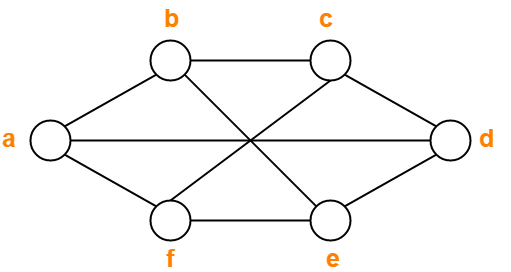
\includegraphics[width=0.5\textwidth]{Graph.png}
\end{center}

You are interested in coloring the nodes of this graph so that no node is adjacent to another node of the same color (thus for example, if node a is red, none of nodes b, d, or f can be red). Suppose that each node can be colored either red, teal, green, or yellow. 
\begin{enumerate}
\item [a)] Formulate an integer program whose solution would minimize the number of colors used. You can formulate as either a concrete or parameterized model. If you formulate a concrete model, do not try writing out all of the constraints, just write enough so that the pattern is clear. \emph{Hint: Just like in problem 1, you need two variables for this problem.}

{\blu

For completeness I'll do both a concrete and parameterized model. First, I'll define some sets that I'll use for both models:

\textbf{\underline{Sets}}

Let $C$ be the set of colors, $C = \{r, t, g, y\}$\\
Let $N$ be the set of nodes, $N = \{a,b,c,d,e,f\}$


Concrete Model:

\textbf{\underline{Decision Variables}}

Let $x_{n,c} = 1$ if node $n$ is assigned color $c$ for $n \in N$ and $c \in C$ \\
Let $z_c = 1$ if color $c$ is used at all for $c \in C$

\textbf{\underline{Objective Function}}

\[
\text{min colors: } z_r + z_t + z_g + z_y
\]

\textbf{\underline{Constraints}}

The following constraints need to be included:
\begin{itemize}
\item Every node must be assigned exactly 1 color
\item Linking constraints for $x$ and $z$ 
\item If a node is a specific color, its neighbors can't be that color
\item Binary
\end{itemize}

Unfortunately, the third one is a ton of constraints, so for the concrete model I'll just do a few. Note that the second constraints can be done in several different ways.

\begin{optprog*}
st & x_{a,r} + x_{a,t} + x_{a,g} + x_{a,y} & = & 1 & \text{(node a is colored)} \\
   & x_{b,r} + x_{b,t} + x_{b,g} + x_{b,y} & = & 1 & \text{(node b is colored)} \\
   & \vdots \\
   & x_{f,r} + x_{f,t} + x_{f,g} + x_{f,y} & = & 1 & \text{(node f is colored)} \\
   & x_{a,r}+x_{b,r} + x_{c,r}+x_{d,r}+x_{e,r}+x_{f,r} & \leq & 6 z_r & \text{(linking red variables)} \\
   & \vdots \\
   & x_{a,y}+x_{b,y} + x_{c,y}+x_{d,y}+x_{e,y}+x_{f,y} & \leq & 6 z_y & \text{(linking yellow variables)} \\
   & x_{a,r} + x_{b,r} & \leq & 1 & \text{(a and b cant both be red)} \\
   & x_{a,t} + x_{b,t} & \leq & 1 & \text{(a and b cant both be teal)} \\
   & \vdots \\
   & x_{e,y} + x_{f,y} & \leq & 1 & \text{(e and f cant both be yellow)} \\
   & x_{a,r}, \dots, x_{f,y} & \in & \{0,1\} & \text{(binary)} \\
   & z_{r}, \dots, z_{y} & \in & \{0,1\} & \text{(binary)} 
\end{optprog*}



\newpage

The parameterized model is a much simpler formulation, except the third constraint is again tough. We need to add the set of edges to our model as well.


\textbf{\underline{Sets}}

Let $C$ be the set of colors\\
Let $N$ be the set of nodes\\
Let $E$ be the set of edges


Concrete Model:

\textbf{\underline{Decision Variables}}

Let $x_{n,c} = 1$ if node $n$ is assigned color $c$ for $n \in N$ and $c \in C$ \\
Let $z_c = 1$ if color $c$ is used at all for $c \in C$

\textbf{\underline{Objective Function}}

\[
\text{min colors: } \sum_{c in C} z_c
\]

\textbf{\underline{Constraints}}

The following constraints need to be included:
\begin{itemize}
\item Every node must be assigned exactly 1 color
\item Linking constraints for $x$ and $z$ 
\item If a node is a specific color, its neighbors can't be that color
\item Binary
\end{itemize}

\begin{optprog*}
st & \sum_{c \in C} x_{n,c} & = & 1 & \text{for $n \in N$} & \text{(each node colored)} \\
   & \sum_{n \in N} x_{n,c} & \leq & |N| z_c & \text{for $c \in C$} & \text{(linking constraints)} \\
   & x_{i,c} + x_{j,c} & \leq & 1 & \text{for $(i,j) \in E$, for $c \in C$} & \text{(neighbor constraints)} \\
   & x_{n,c} , z_c & \in & \{0,1\} & \text{for $n \in N$ for $c \in C$} & \text{(binary)} 
\end{optprog*}

}


\item [b)] How many total constraints does this model have?

{\blu

For this problem, we have 4 colors, 6 nodes, and 9 edges

Of the four types of constraints we have:
\begin{enumerate}
\item Each node is assigned 1 color. We have 1 constraint for each node, so 6 total constraints.
\item Linking constraints. If you do this my way, we have one constraint for each color so we have 4 constraints. Your model may have 24 of these constraints if you formulate them as $x_{n,c} \leq z_c$.
\item Neighbor constraint. For each edge, we have a constraint for each color. So there are 9 edges and 4 colors; thus, we have $9*4=36$ constraints.
\item Binary: One constraint for each variable, so we have 24 $x$ variables and 4 $z$ variables giving us 28 constraints.
\end{enumerate}


Thus, all together we have $6+4+36+28=74$ constraints. 

}

\end{enumerate}







\end{document}
